\title{Curs 2: Grafuri Euler; Grafuri Hamilton}
\date{Bălți, 2013}

\begin{document}

\maketitle

\begin{frame}
  \frametitle{Problema poștașului chinez}

\pause

Pentru prima dată problema a fost publicată de matematicianul chinez Mei-Ko Kwan (1962).

De aici și denumirea problemei.

\end{frame}

\begin{frame}
  \frametitle{Ciclu Euler; Graf Euler}

Un ciclu simplu, dintr-un graf conex, care conține toate muchiile grafului se numește \emph{ciclu Euler} (sau \emph{ciclu eulerian}).
\pause

Un graf care conține cel puțin un ciclu Euler se numește \emph{graf Euler} (sau \emph{graf eulerian}).
\pause

\alert{În aplicații este utilă următoarea remarcă:} într-un ciclu eulerian nu este permisă repetiția muchiilor, dar se pot repeta vîrfurile.
\pause

\end{frame}

\begin{frame}
  \frametitle{Exemple}

\begin{figure}
\centering%
\begin{tikzpicture}
  \SetVertexMath

  \begin{scope}
    \mygrComet
  \end{scope}

  \begin{scope}[shift={(6,0)}]
    \mygrComet
    \Edge[style={bend right,in=-90,out=-90}](u0)(v2)
    \Edge(v1)(v3)
  \end{scope}
\end{tikzpicture}
\end{figure}
\pause

Primul graf (de la stînga spre dreapta) nu este Euler, iar al doilea este Euler. 
\pause

\begin{figure}
\centering%
\begin{tikzpicture}
  \SetVertexMath

  \begin{scope}
    \mygrComet
    \Edge[style={bend right,in=-90,out=-90}](u0)(v2)
    \Edge(v1)(v3)
    \SetUpEdge[style={->,ultra thick},color=red]
    \Edges(u0,v1,v0,v3,v2,v1,v3,u0,u1,v2)
    \Edge[style={in=-90,out=-90,->,ultra thick},color=red](v2)(u0)
  \end{scope}
\end{tikzpicture}
\caption{Ciclul $(u0,v1,v0,v3,v2,v1,v3,u0,u1,v2)$ este eulerian.}
\end{figure}
 
\end{frame}

\begin{frame}
  \frametitle{Lanț Euler; Graf semi-Euler}

Într-un graf conex, un lanț simplu care conține toate muchiile grafului se numește \emph{lanț Euler} (sau \emph{lanț eulerian}).
\pause

Un graf care conține cel puțin un lanț Euler se numește \emph{graf semi-Euler} (sau \emph{graf semi-eulerian}).
\pause

Un lanț eulerian se mai numește \emph{traseu eulerian}.

\end{frame}

\begin{frame}
  \frametitle{Exemple}

\begin{figure}
\centering%
\begin{tikzpicture}
  \SetVertexMath

  \begin{scope}
    \mygrComet
  \end{scope}

  \begin{scope}[shift={(6,0)}]
    \mygrComet
    %\Edge[style={bend right,in=-90,out=-90}](u0)(v2)
    \Edge(v1)(v3)
  \end{scope}
\end{tikzpicture}
\end{figure}
\pause

Primul graf (de la stînga spre dreapta) nu este semi-Euler, iar al doilea este semi-Euler. 
\pause

\begin{figure}
\centering%
\begin{tikzpicture}
  \SetVertexMath

  \begin{scope}
    \mygrComet
    \Edge(v1)(v3)
    \SetUpEdge[style={->,ultra thick},color=red]
    \Edges(u0,v1,v0,v3,v2,v1,v3,u0,u1,v2)
  \end{scope}
\end{tikzpicture}
\caption{Lanțul $(u0,v1,v0,v3,v2,v1,v3,u0,u1,v2)$ este semi-eulerian.}
\end{figure}

\end{frame}


\begin{frame}
  \frametitle{Condiție necesară și suficientă}

\begin{theorem}[Euler]
Un graf conex este eulerian dacă şi numai dacă oricare vîrf al său are gradul par.
\end{theorem}
\pause

\begin{theorem}
Un graf conex este semi-eulerian dacă şi numai dacă cel mult două vîrfuri ale sale au grad impar.
\end{theorem}

\end{frame}

\begin{frame}
  \frametitle{Eulerizare}

Grafurile care nu sînt euleriene pot fi transformate în grafuri euleriene.
Dublînd unele muchii existente putem face ca toate vîrfurile să aibă grad par.
Graful obținut va fi eulerian. 
Iar procedeul de dublare a muchiilor cu scopul de a obține un graf eulerian se numește \emph{eulerizare}.
\pause

\alert{Nu este permis adăugare de muchii între vîrfurile care nu-s vecine}; este permis doar dublarea muchiilor existente.
\pause

O euleriazare se numește \emph{bună} dacă conține numărul minim de muchii noi.
\pause

Numărul minim de muchii necesare pentru eulerizarea unui graf $G$ se numește \emph{numărul de eulerizare} și se notează $ecc(G)$.
\end{frame}

\begin{frame}
  \frametitle{Eulerizare}

\begin{figure}
\centering%
\begin{tikzpicture}
  \SetVertexMath

  \begin{scope}
    \mygrComet
  \end{scope}
\end{tikzpicture}
\end{figure}
\pause

Graful de mai sus, nefiind Euler, poate fi eulerizat în felulurile următoare:
\pause

\begin{figure}
\centering%
\begin{tikzpicture}
  \SetVertexNoLabel

  \begin{scope}
    \mygrComet
    \Edge[style={bend right}](v2)(v1)
    \Edge[style={bend right}](u0)(v3)
  \end{scope}

  \begin{scope}[shift={(6,0)}]
    \mygrComet
    \Edge[style={bend right}](v2)(v1)
    \Edge[style={bend left}](v2)(v3)
    \Edge[style={bend right,out=100,in=80}](v2)(u1)
    \Edge[style={bend right,out=100,in=80}](u1)(u0)
  \end{scope}
\end{tikzpicture}
\end{figure}

\end{frame}

\begin{frame}
  \frametitle{Problema Comis-Voiajorului}

\end{frame}

\begin{frame}
  \frametitle{Ciclu Hamilton; Graf Hamilton}

Un ciclu elementar, dintr-un graf conex, care conține toate vîrfurile grafului se numește \emph{ciclu Hamilton} (sau \emph{ciclu hamiltonian}).
\pause

Un graf care conține cel puțin un ciclu Hamilton se numește \emph{graf Hamilton} (sau \emph{graf hamiltonian}).
\pause

\alert{În aplicații este utilă următoarea remarcă:} un ciclu hamiltonian trebuie treacă prin toate vîrfurile grafului, dar nu și prin toate muchiile.

\end{frame}

\begin{frame}
  \frametitle{Exemple}

\begin{figure}
\centering%
\begin{tikzpicture}
  \SetVertexMath

  \begin{scope}
    \mygrComet
  \end{scope}

  \begin{scope}[shift={(6,0)}]
    \mygrHouse
  \end{scope}
\end{tikzpicture}
\end{figure}
\pause

Primul graf (de la stînga spre dreapta) este Hamilton, iar al doilea nu este Hamilton. 
\pause

\begin{figure}
\centering%
\begin{tikzpicture}
  \SetVertexMath

  \begin{scope}
    \mygrComet
    \SetUpEdge[style={->,ultra thick},color=red]
    \Edges(u0,u1,v2,v1,v0,v3,u0)
  \end{scope}

\end{tikzpicture}
\end{figure}
 
\end{frame}

\begin{frame}
  \frametitle{Ciclu Hamilton; Graf Hamilton}

Evident, grafurile $C_n$ sînt hamiltoniene, pentru orice $n$; grafurile $K_n$ sînt hamiltoniene pentru $n\geq 3$.

\end{frame}

\begin{frame}
  \frametitle{Lanț Hamilton; Graf semi-Hamilton}

Într-un graf conex, un lanț elementar care conține toate vîrfurile grafului se numește \emph{lanț Hamilton} (sau \emph{lanț hamiltonian}).

Un graf care conține cel puțin un lanț Hamilton se numește \emph{graf semi-Hamilton} (sau \emph{graf semi-hamiltonian}).

\end{frame}

\begin{frame}
  \frametitle{Exemple}

\begin{figure}
\centering%
\begin{tikzpicture}
  \SetVertexMath

  \begin{scope}
    \mygrHouse
  \end{scope}

\end{tikzpicture}
\end{figure}
\pause

Graful de mai sus este semi-hamiltonian. 
\pause

\begin{figure}
\centering%
\begin{tikzpicture}
  \SetVertexMath

  \begin{scope}
    \mygrHouse
    \SetUpEdge[style={->,ultra thick},color=red]
    \Edges(z,x,u,v,y)
  \end{scope}
\end{tikzpicture}
\end{figure}

\end{frame}

\begin{frame}
  \frametitle{Condiții suficiente}

\begin{theorem}[Ore]
Dacă $G$ este un graf simplu cu $|G| = n \geq 3$ și pentru orice două vîrfuri 
neadiacente $u$ și $v$ avem 
\begin{equation}\label{ore_1960_sum}
 d(u)+d(v)\geq n, 
\end{equation}
atunci $G$ este Hamilton.
\end{theorem}


\end{frame}

\begin{frame}
  \frametitle{Teorema Ore}

\begin{proof}

Presupunem (prin absurd) că teorema este falsă.\pause

Adică există un graf pe $n$ vîrfuri, $n\geq 3$, care verifică condițiile teoremei însă nu este hamiltonian.\pause

Dacă astfel de grafuri sînt mai multe (toate pe $n$ vîrfuri) alegem graful cu cel mai mare număr de muchii; notăm acest graf prin $G$.\pause

Fie $p$ și $q$ două vîrfuri neadiacente ale grafului $G$; în virtutea condiției de maximalitate a lui $G$, $G+pq$ este hamiltonian.\pause

Mai mult, muchia $pq$ trebuie să aparțină oricărui ciclu hamiltonian din $G+pq$ deoarece în caz contrar am avea un ciclu hamiltonian în $G$.\pause

În același timp: $d(p)+d(q)\geq n$.

\end{proof}


\end{frame}

\begin{frame}
  \frametitle{Teorema Ore}

\begin{proof}[Demonstrație; Continuare]

Fie un oarecare ciclu hamiltonian în $G+xy$:
\begin{equation}\label{demonstratia-teoremei-lui-ore-ciclu-hamilton-alest-arbitrar}
  p,v_1,v_2,...,v_{n-2},q,p.
\end{equation}\pause

Observăm că dacă $v_i$ este adiacent cu $p$ atunci $v_{i-1}$ nu poate fi adiacent cu $q$; în caz contrar ciclul:
\[
  p,v_1,v_2,v_{i-1},q,v_{n-2},v_{n-3},v_{n-4},...,v_{i},p
\]
este hamiltonian în $G$.\pause

\begin{figure}
\centering%
\begin{tikzpicture}
  \SetUpVertex[Lpos=-45]
  \Vertex[L=$p$]{p}
  \Vertex[x=1,y=0,L=$v_1$]{v1}
  \Vertex[x=3,y=0,L=$v_{i-1}$]{vi1}
  \Vertex[x=4,y=0,L=$v_i$]{vi}
  \Vertex[x=6,y=0,L=$v_{n-2}$]{vn2}
  \Vertex[x=7,y=0,L=$q$]{q}
  
  \Edges(p,v1)
  \Edges(vi1,vi)
  \Edges(vn2,q)
  \Edge[style={bend left}](p)(vi)
  \Edge[style={bend left}](vi1)(q)
  \SetUpEdge[style={dashed}]
  \Edge(v1)(vi1)
  \Edge(vi)(vn2)
\end{tikzpicture}
\end{figure}


\end{proof}

\end{frame}


\begin{frame}
  \frametitle{Teorema Ore}

\begin{proof}[Demonstrație; Continuare]
Din cele de mai sus reiese că, întrucît în $G$ sînt $d(p)$ vîrfuri adiacente cu $p$, trebuie să fie cel puțin $d(p)+1$ vîrfuri neadiacente cu $q$. 
\pause

Așadar
\[
  \begin{array}{ll}
    d(p)+d(q)	&\leq	d(p) + (n - d(p) - 1)\\
		&=	n-1\\
  \end{array}
\]

\end{proof}

\end{frame}

\begin{frame}
  \frametitle{Condiții suficiente}

\begin{theorem}[Dirac]
Dacă $G$ este un graf simplu cu $|G| = n \geq 3$ și $\delta(G)\geq\frac{n}{2}$, 
atunci $G$ este Hamilton.
\end{theorem}
\pause

Teorema Dirac poate fi demonstrată ca un corolar al teoremei Ore.

Dar istoric, întîi a fost publicată acestă teoremă și doar peste cîțiva ani a fost publicată teorema Ore. 
\pause

Pe de altă parte ambele teoreme sînt generalizate de următoarea teoremă:
\pause

\begin{theorem}[Pos\' a]
Dacă $G$ este un graf simplu cu $|G| = n \geq 3$ și pentru orice $k$, $1\leq k\leq \frac{n-1}{2}$, numărul de vîrfuri cu grad mai mica sau egal cu $k$ nu întrece $k$.
\end{theorem}



\end{frame}

\begin{frame}
  \frametitle{Condiții necesare}

\begin{theorem}
Dacă un graf bipartit cu bipartiția $\{X,Y\}$ este hamiltonian atunci $|X|=|Y|$; 
dacă graful este semi-hamiltonian atunci $||X|-|Y||\leq 1$.
\end{theorem}
\pause

\begin{proof}
Fie $G$ un graf bipartit cu bipartiția $\{X,Y\}$.
\pause

Presupunem că $G$ conține un lanț hamiltonian:
\[
  v_1,v_2,...,v_n.
\]
\pause
 
Dacă $v_1\in X$ atunci $v_2\in Y$, $v_3\in X$, $v_4\in Y$ etc.

\end{proof}


\end{frame}

\begin{frame}
  \frametitle{Condiții necesare}

\begin{proof}[Demonstrație; Continuare]
Așadar $X=\{v_1,v_3,...\}$ (vîrfurile cu indice impar) și $Y=\{v_2,v_4,...\}$ (vîrfurile cu indice par).
\pause

Rezultă că, dacă $n$ este par atunci $|X|=|Y|=\frac{n}{2}$; dacă $n$ este impar atunci $|X|=\frac{n+1}{2}$, iar $|Y|=\frac{n-1}{2}$.
\pause

În ambele cazuri diferența dintre $|X|$ și $|Y|$ este cel mult 1.
\pause

Dacă $G$ conține un ciclu hamiltonian și $v_1\in X$, atunci $v_n\in Y$; adică $n$ este par și $|X|=|Y|$.
\end{proof}
\end{frame}

\begin{frame}
  \frametitle{Secvențe de grade hamiltoniene}

\begin{definition}
O secvență $(a_1,a_2,...,a_n)$ de numere naturale se numeste \emph{hamiltoniană} dacă orice graf pe $n$ vîrfuri cu secvența de grade mai mare sau egală punctual decît $(a_1,a_2,...,a_n)$ este hamiltonian.
\end{definition}
\pause

O secvență $(b_1,b_2,...,b_n)$ de numere naturale este mai mare sau egală punctual decît altă secvență $(a_1,a_2,...,a_n)$ [de numere naturale], dacă $b_i\geq a_i$, $1\leq i\leq n$.


\end{frame}

\begin{frame}
  \frametitle{Condiții suficiente și necesare}

\begin{theorem}[Chvátal]
O secvență $(d_1,d_2,...,d_n)$ de numere naturale, $n\geq 3$, este hamiltoniană dacă și numai dacă 
\[
  d_i\leq i \Rightarrow d_{n-1}\geq n-i,\quad \forall i< \frac{n}{2}.
\]

\end{theorem}

\end{frame}


\begin{frame}
  \frametitle{Secvențe de grade semi-hamiltoniene}

\begin{definition}
O secvență $(d_1,d_2,...,d_n)$ de numere naturale se numeste \emph{semi-hamiltoniană} dacă orice graf pe $n$ vîrfuri cu secvența de grade mai mare sau egală punctual decît $(d_1,d_2,...,d_n)$ este semi-hamiltonian.
\end{definition}
\pause

\begin{corollary}
O secvență $(d_1,d_2,...,d_n)$ de numere naturale, $n\geq 2$ și $0\leq d_1\leq d_2\leq ...\leq d_n < n$ este semi-hamiltoniană dacă și numai dacă 
\[
  d_i< i \Rightarrow d_{n+1-i}\geq n-i,\quad \forall i\leq \frac{n}{2}.
\] 
\end{corollary}


\end{frame}

\begin{frame}
  \frametitle{Închiderea [unui graf]}

\begin{definition}
Fiind dat un graf $G$, numim \emph{închiderea} lui $G$, notată prin $cl(G)$, graful obținut prin aplicarea recursivă a următorului algoritm:
\begin{enumerate}
 \item orice două vîrfuri neadiacente $u$ și $v$ cu $d(u)+d(v)\geq n$ se unesc printr-o muchie;
 \item pasul anterior se aplică atîta timp cît există astfel de vîrfuri.
\end{enumerate}
\end{definition}

\end{frame}

\begin{frame}
  \frametitle{Închiderea}

\begin{figure}
\centering%
\begin{tikzpicture}
  \SetVertexMath

  \begin{scope}
    \mygrComet
    \draw (2,-1.7) node (G){$G$; $|G|=6$};
  \end{scope} 

  \draw[->,ultra thick,line width=0.5mm] (5,0) -- (5.5,0);

  \begin{scope}[shift={(6,0)}]
    \mygrComet
    \Edge(v1)(v3)
    \draw (2,-1.7) node (v1v3G){$d(v_1)+d(v_3)\geq 6$};
  \end{scope}

  \draw[->,ultra thick,line width=0.5mm] (-1,-3.5) -- (-0.5,-3.5);

  \begin{scope}[shift={(0,-3.5)}]
    \mygrComet
    \Edge(v1)(v3)
    \Edge[style={bend left}](u1)(v1)
    \draw (2,-1.7) node (u1v1G){$d(u_1)+d(v_1)\geq 6$};
  \end{scope} 

  \draw[->,ultra thick,line width=0.5mm] (5,-3.5) -- (5.5,-3.5);

  \begin{scope}[shift={(6,-3.5)}]
    \mygrComet
    \Edge(v1)(v3)
    \Edge[style={bend left}](u1)(v1)
    \Edge[style={bend right}](u1)(v3)
    \draw (2,-1.7) node (u1v3G){$d(u_1)+d(v_3)\geq 6$};
  \end{scope}

\end{tikzpicture}
\end{figure}

\end{frame}


\begin{frame}
  \frametitle{Închiderea}

\begin{figure}
\centering%
\begin{tikzpicture}
  \SetVertexMath

  \draw[->,ultra thick,line width=0.5mm] (-1,0) -- (-0.5,0);

  \begin{scope}[shift={(0,0)}]
    \mygrComet
    \Edge(v1)(v3)
    \Edge[style={bend left}](u1)(v1)
    \Edge[style={bend right}](u1)(v3)
    \Edge[style={bend right}](u0)(v2)
    \draw (2,-1.7) node (u0v2G){$d(u_0)+d(v_2)\geq 6$};
  \end{scope}

  \draw[->,ultra thick,line width=0.5mm] (5,0) -- (5.5,0);

  \begin{scope}[shift={(6,0)}]
    \mygrComet
    \Edge(v1)(v3)
    \Edge[style={bend left}](u1)(v1)
    \Edge[style={bend right}](u1)(v3)
    \Edge[style={bend right}](u0)(v2)
    \Edge[style={bend right}](u0)(v0)
    \Edge[style={bend right}](u1)(v0)
    \draw (2,-1.7) node (u1v0G){$d(u_1)+d(v_0)\geq 6$};
  \end{scope}

  \draw[->,ultra thick,line width=0.5mm] (-1,-3.5) -- (-0.5,-3.5);

  \begin{scope}[shift={(0,-3.5)}]
    \mygrComet
    \Edge(v1)(v3)
    \Edge[style={bend left}](u1)(v1)
    \Edge[style={bend right}](u1)(v3)
    \Edge[style={bend right}](u0)(v2)
    \Edge[style={bend right}](u0)(v0)
    \Edge[style={bend right}](u1)(v0)
    \Edge(v2)(v0)
    \draw (2,-1.7) node (v2v0G){$d(v_2)+d(v_0)\geq 6$};
  \end{scope} 

  \draw[<-,ultra thick,line width=0.5mm] (5,-3.5) -- (5.5,-3.5);
  \draw (7, -3.5) node (clG){$cl(G)$} ;

\end{tikzpicture}
\end{figure}

\end{frame}


\begin{frame}
  \frametitle{Închiderea}

\begin{figure}
\centering%
\begin{tikzpicture}
  \SetVertexMath

  \begin{scope}
    \mygrHouse
    \draw (1,-2) node (G){$G$; $|G|=5$};
  \end{scope}

  \draw[->,ultra thick,line width=0.5mm] (3.5,0) -- (4.5,0);

 \begin{scope}[shift={(6,0)}]
    \mygrHouse
    \draw (1,-2) node (clG){$cl(G)$};
  \end{scope}

\end{tikzpicture}
\end{figure}

\end{frame}


\begin{frame}
  \frametitle{Condiții suficiente și necesare}

\begin{theorem}[Bondy-Chvátal]
Un graf $G$ este hamiltonian dacă și numai dacă $cl(G)$ este hamiltonian.
\end{theorem}
\pause

\begin{corollary}
Dacă închiderea unui graf $G$ este graf complet atunci $G$ este hamiltonian.
\end{corollary}


\end{frame}

\begin{frame}
  \frametitle{Graful liniilor}

\emph{Graful liniilor} al unui grafului $G$  este graful $L(G)$ pe $E(G)$ în care două vîrfuri sînt vecine dacă și numai dacă muchiile corespunzătoare în $G$ sînt vecine.
\pause

\begin{figure}
\centering%
\begin{tikzpicture}
  \SetVertexNoLabel
  \grEmptyCycle[RA=1]{4}
    \Edge[label=e](a0)(a1)
    \Edge[label=f](a2)(a3)    
    \Edge[label=g](a0)(a3)
    \draw (0,-2) node (G){$G$}; 
    
  \begin{scope}[shift={(4,0)}]
    \SetVertexLabel
    \Vertices{circle}{e,f,g}
    \Edges(e,g,f)
      \draw (0,-2) node (LG){$L(G)$};
  \end{scope}  
\end{tikzpicture}
\end{figure}
 
\end{frame}

\begin{frame}
  \frametitle{Graful liniilor}

Orice ciclu eulerian din $G$ se transformă într-un ciclu hamiltonian în $L(G)$.
\pause

\begin{theorem}
  Dacă un graf $G$ este eulerian atunci graful liniilor $L(G)$ este hamiltonian.
\end{theorem}

\end{frame}

\end{document}

